\section{Controlled Pendulum System}
\label{sec:case_study_controlled_pendulum_system}

The case-study system is a closed-loop controlled pendulum with sensor feedback, actuator dynamics, and contact-enabled plant variants.
Figure~\ref{fig:case_controlled_pendulum_system} shows the signal flow used in the co-simulation scenarios.
The setpoint block generates the reference angle.
The angle sensor and decoder provide the measured feedback angle.
The PID controller computes the drive command.
The drive maps this command to the actuator torque applied to the pendulum plant.

The main continuous input signals are the reference angle \(\theta_{\mathrm{ref}}\), the measured feedback angle \(\theta_{\mathrm{meas}}\), the control signal \(u_{\mathrm{control}}\), and the actuator torque \(\tau\).
The plant outputs used in the case study are the pendulum angle \(\theta\) and the angular velocity \(\omega\).
The contact event is a discrete signal emitted by the pendulum plant when wall contact occurs.
In contact scenarios, this event triggers the pendulum contact response and the reset of the PID integrator.

\begin{landscape}
\begin{figure}[p]
  \centering
  \vspace{-1ex}
  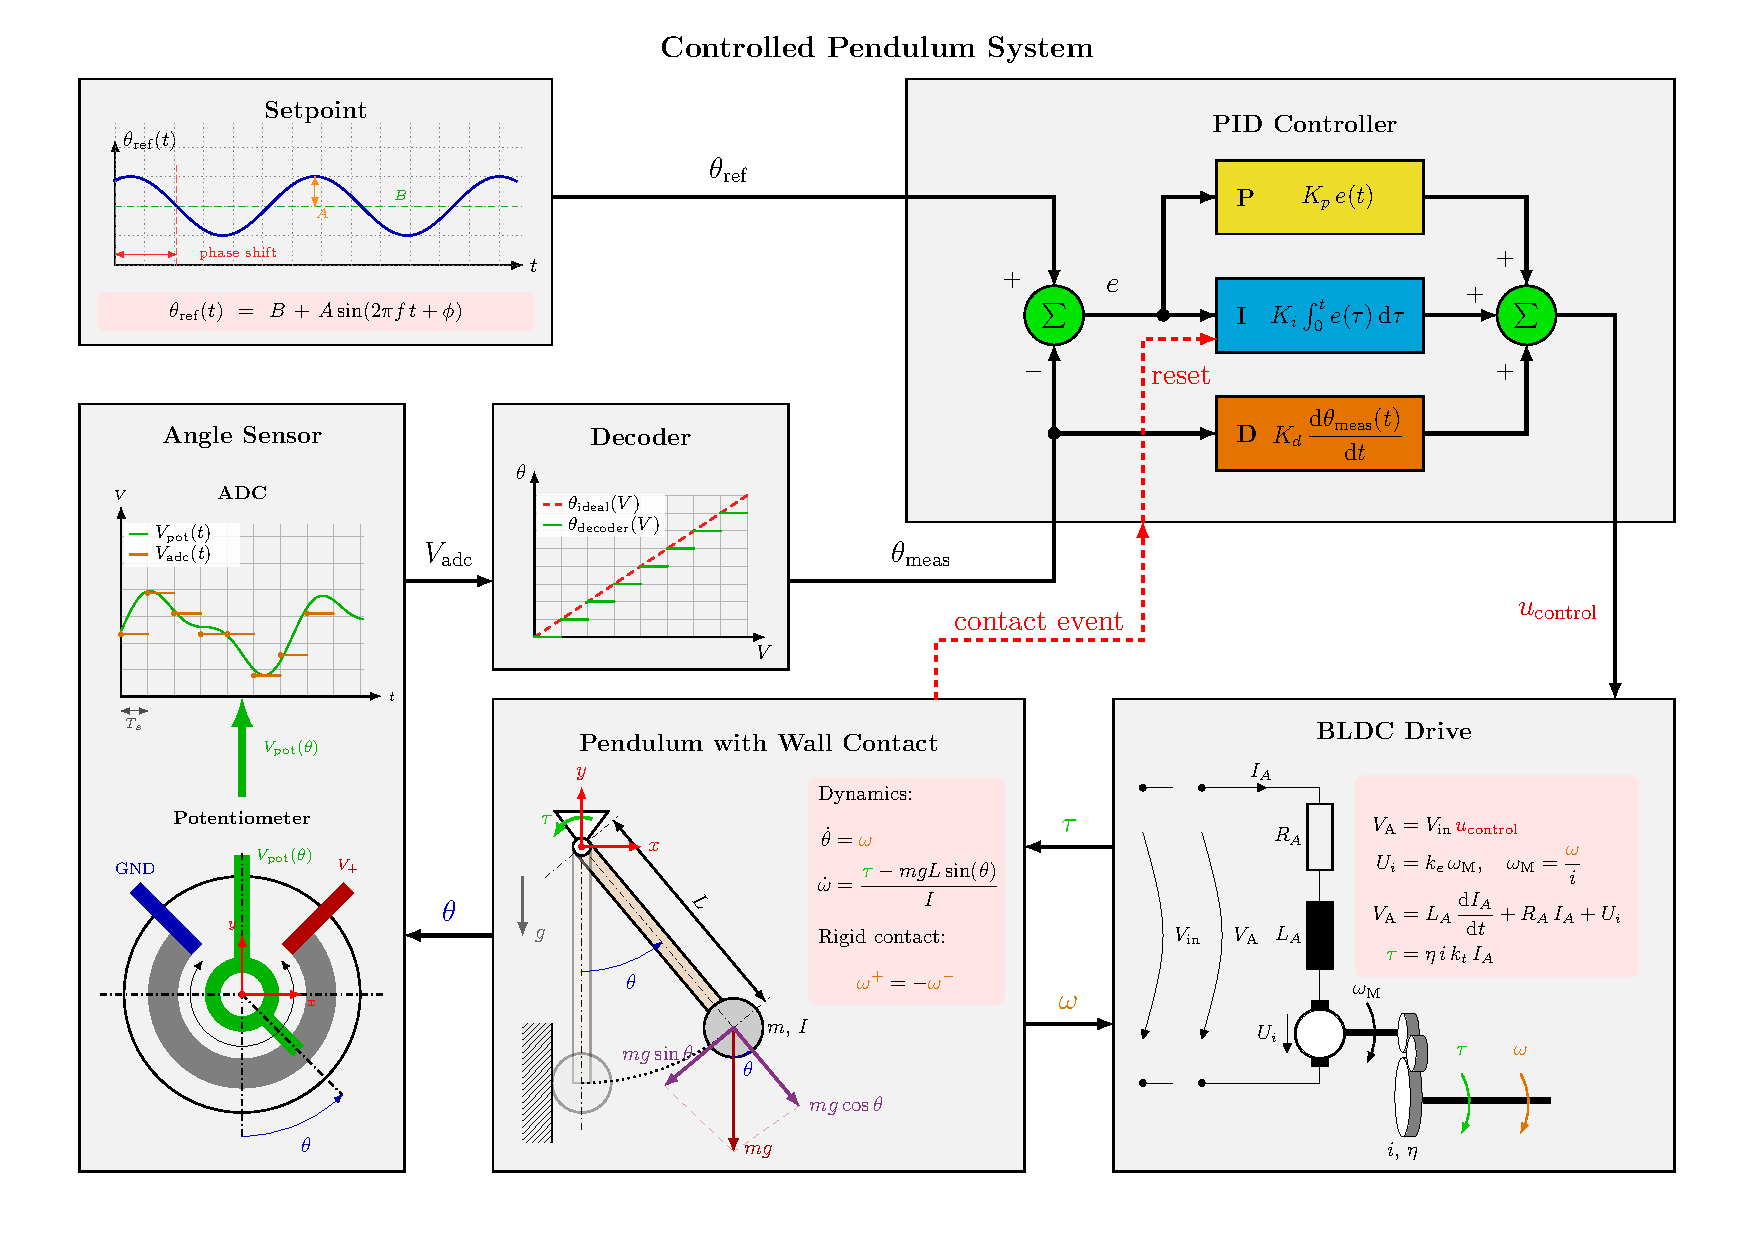
\includegraphics[
    width=\linewidth,
    height=0.95\textheight,
    keepaspectratio
  ]{figures/6_case_study/controlled_pendulum/system_assembly.pdf}
  \vspace{-5ex}
  \caption[Closed-loop signal flow of the controlled-pendulum case study]{Closed-loop signal flow of the controlled-pendulum case study.
  The pendulum plant is the interchangeable subsystem used by the FMU, OpenSim, FEM, and \texttt{MasterPendulum} variants.}
  \label{fig:case_controlled_pendulum_system}
\end{figure}
\end{landscape}

Table~\ref{tab:case_study_subsystems} summarizes the subsystem roles used in the validation scenarios.
It lists only the information needed to understand the closed-loop signal flow.
Model-specific details of the pendulum variants are introduced in Section~\ref{sec:case_study_pendulum_models}.

\begin{table}[tbp]
    \centering
    \small
    \caption{Subsystems of the controlled-pendulum case study.}
    \label{tab:case_study_subsystems}
    \begin{tabular}{p{3.0cm}p{5.0cm}p{5.6cm}}
        \toprule
        \textbf{Subsystem} & \textbf{Role in the closed loop} & \textbf{Use in the case study} \\
        \midrule
        Setpoint
        & Generates the reference angle \(\theta_{\mathrm{ref}}\)
        & Defines the motion for all scenarios \\
        \addlinespace
        Angle sensor and decoder
        & Converts the plant angle into the feedback signal \(\theta_{\mathrm{meas}}\)
        & Used as exact or quantized feedback path depending on the scenario \\
        \addlinespace
        PID controller
        & Computes the normalized drive command \(u_{\mathrm{control}}\)
        & The reset-capable variant clears the integrator state after contact \\
        \addlinespace
        Drive
        & Maps the controller command and shaft speed to the actuator torque \(\tau\)
        & The dynamic drive is used in the reported scenarios \\
        \addlinespace
        Pendulum plant
        & Receives the actuator torque and returns \(\theta\), \(\omega\), and contact events
        & Exchanged between FMU, OpenSim, FEM, and \texttt{MasterPendulum} variants \\
        \bottomrule
    \end{tabular}
\end{table}

All pendulum variants implement the same plant interface.
The input is the actuator torque \(\tau\).
The required outputs are the angle \(\theta\), the angular velocity \(\omega\), and the contact event.
This interface allows the FMU, OpenSim, FEM, and multi-model pendulum variants to be exchanged without changing the controller, drive, sensor, or decoder.

The following sections separate the system architecture from the pendulum models.
Section~\ref{sec:case_study_pendulum_models} describes how the individual pendulum variants realize the shared interface.
The validation scenarios later reuse the same closed-loop structure and change only the active pendulum model, the contact configuration, or the communication step size.
